\documentclass[tikz]{standalone}
\usepackage{pgfplots}
\pgfplotsset{compat=1.15}
\usepackage{mathrsfs}
\usetikzlibrary{arrows,calc}
\usepackage{tkz-euclide}

\usepackage{fp}
\pagestyle{empty}

\definecolor{AngleClr}{rgb}{0,0.39215686274509803,0}
\definecolor{ShapeClr}{rgb}{0.6,0.2,0}

\begin{document}

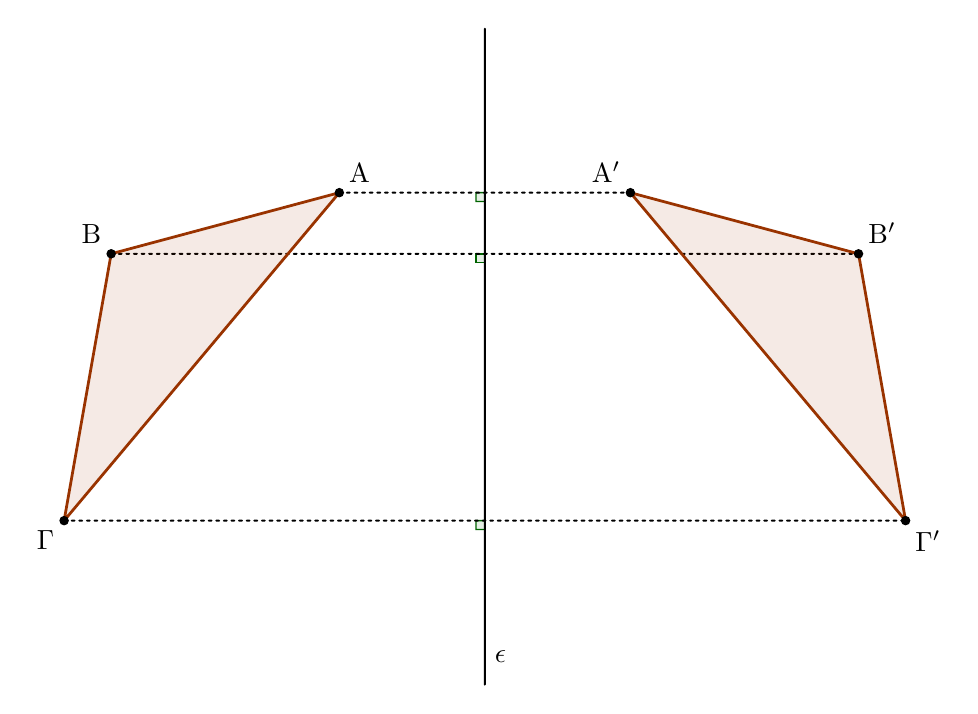
\begin{tikzpicture}[scale=.75]
\tkzSetUpLine[line width=1pt,color=black]
\tkzSetUpPoint[fill=black]

\tkzDefPoint(75:4){A}
\tkzDefPoint(135:4){B}
\tkzDefPoint(205:4){C}
\tkzDefPoints{3.5/2.5/O1,3.5/-4/O2}

\tkzDefPointBy[reflection=over O1--O2](A){} \tkzGetPoint{A'}
\tkzDefPointBy[reflection=over O1--O2](B){} \tkzGetPoint{B'}
\tkzDefPointBy[reflection=over O1--O2](C){} \tkzGetPoint{C'}

\tkzDefMidPoint(A,A') \tkzGetPoint{OA}
\tkzDefMidPoint(B,B') \tkzGetPoint{OB}
\tkzDefMidPoint(C,C') \tkzGetPoint{OC}

\tkzMarkRightAngles[line width=0.5pt, size=.15,color=AngleClr,fill=AngleClr,fill opacity=0.1](A,OA,O2 B,OB,O2 C,OC,O2)

\tkzDrawSegments[line width=0.75pt,color=black,dashed,dash pattern=on 1pt off 1.75pt](A,A' B,B' C,C')

\tkzDrawSegment[line width=0.75pt,color=black,add=0.5 and 0.5](OA,OC)

\tkzFillPolygon[fill=ShapeClr,fill opacity=0.1](A,B,C)
\tkzFillPolygon[fill=ShapeClr,fill opacity=0.1](A',B',C')
\tkzDrawPolygon[color=ShapeClr](A,B,C)
\tkzDrawPolygon[color=ShapeClr](A',B',C')

\tkzDrawPoints[size=3](A,B,C,A',B',C')
\tkzLabelPoint[above right](A){$\rm A$}
\tkzLabelPoint[above left](B){$\rm B$}
\tkzLabelPoint[below left](C){$\rm \Gamma$}

\tkzLabelPoint[above left](A'){$\rm A'$}
\tkzLabelPoint[above right](B'){$\rm B'$}
\tkzLabelPoint[below right](C'){$\rm \Gamma'$}

\tkzLabelPoint[right](O2){$\rm \epsilon$}


\end{tikzpicture}

\end{document}
